\documentclass[twoside]{book}

% Packages required by doxygen
\usepackage{fixltx2e}
\usepackage{calc}
\usepackage{doxygen}
\usepackage[export]{adjustbox} % also loads graphicx
\usepackage{graphicx}
\usepackage[utf8]{inputenc}
\usepackage{makeidx}
\usepackage{multicol}
\usepackage{multirow}
\PassOptionsToPackage{warn}{textcomp}
\usepackage{textcomp}
\usepackage[nointegrals]{wasysym}
\usepackage[table]{xcolor}

% Font selection
\usepackage[T1]{fontenc}
\usepackage[scaled=.90]{helvet}
\usepackage{courier}
\usepackage{amssymb}
\usepackage{sectsty}
\renewcommand{\familydefault}{\sfdefault}
\allsectionsfont{%
  \fontseries{bc}\selectfont%
  \color{darkgray}%
}
\renewcommand{\DoxyLabelFont}{%
  \fontseries{bc}\selectfont%
  \color{darkgray}%
}
\newcommand{\+}{\discretionary{\mbox{\scriptsize$\hookleftarrow$}}{}{}}

% Page & text layout
\usepackage{geometry}
\geometry{%
  a4paper,%
  top=2.5cm,%
  bottom=2.5cm,%
  left=2.5cm,%
  right=2.5cm%
}
\tolerance=750
\hfuzz=15pt
\hbadness=750
\setlength{\emergencystretch}{15pt}
\setlength{\parindent}{0cm}
\setlength{\parskip}{3ex plus 2ex minus 2ex}
\makeatletter
\renewcommand{\paragraph}{%
  \@startsection{paragraph}{4}{0ex}{-1.0ex}{1.0ex}{%
    \normalfont\normalsize\bfseries\SS@parafont%
  }%
}
\renewcommand{\subparagraph}{%
  \@startsection{subparagraph}{5}{0ex}{-1.0ex}{1.0ex}{%
    \normalfont\normalsize\bfseries\SS@subparafont%
  }%
}
\makeatother

% Headers & footers
\usepackage{fancyhdr}
\pagestyle{fancyplain}
\fancyhead[LE]{\fancyplain{}{\bfseries\thepage}}
\fancyhead[CE]{\fancyplain{}{}}
\fancyhead[RE]{\fancyplain{}{\bfseries\leftmark}}
\fancyhead[LO]{\fancyplain{}{\bfseries\rightmark}}
\fancyhead[CO]{\fancyplain{}{}}
\fancyhead[RO]{\fancyplain{}{\bfseries\thepage}}
\fancyfoot[LE]{\fancyplain{}{}}
\fancyfoot[CE]{\fancyplain{}{}}
\fancyfoot[RE]{\fancyplain{}{\bfseries\scriptsize Generated by Doxygen }}
\fancyfoot[LO]{\fancyplain{}{\bfseries\scriptsize Generated by Doxygen }}
\fancyfoot[CO]{\fancyplain{}{}}
\fancyfoot[RO]{\fancyplain{}{}}
\renewcommand{\footrulewidth}{0.4pt}
\renewcommand{\chaptermark}[1]{%
  \markboth{#1}{}%
}
\renewcommand{\sectionmark}[1]{%
  \markright{\thesection\ #1}%
}

% Indices & bibliography
\usepackage{natbib}
\usepackage[titles]{tocloft}
\setcounter{tocdepth}{3}
\setcounter{secnumdepth}{5}
\makeindex

% Hyperlinks (required, but should be loaded last)
\usepackage{ifpdf}
\ifpdf
  \usepackage[pdftex,pagebackref=true]{hyperref}
\else
  \usepackage[ps2pdf,pagebackref=true]{hyperref}
\fi
\hypersetup{%
  colorlinks=true,%
  linkcolor=blue,%
  citecolor=blue,%
  unicode%
}

% Custom commands
\newcommand{\clearemptydoublepage}{%
  \newpage{\pagestyle{empty}\cleardoublepage}%
}

\usepackage{caption}
\captionsetup{labelsep=space,justification=centering,font={bf},singlelinecheck=off,skip=4pt,position=top}

%===== C O N T E N T S =====

\begin{document}

% Titlepage & ToC
\hypersetup{pageanchor=false,
             bookmarksnumbered=true,
             pdfencoding=unicode
            }
\pagenumbering{alph}
\begin{titlepage}
\vspace*{7cm}
\begin{center}%
{\Large Meine Projekt }\\
\vspace*{1cm}
{\large Generated by Doxygen 1.8.14}\\
\end{center}
\end{titlepage}
\clearemptydoublepage
\pagenumbering{roman}
\tableofcontents
\clearemptydoublepage
\pagenumbering{arabic}
\hypersetup{pageanchor=true}

%--- Begin generated contents ---
\chapter{Hierarchical Index}
\section{Class Hierarchy}
This inheritance list is sorted roughly, but not completely, alphabetically\+:\begin{DoxyCompactList}
\item Q\+Graphics\+Rect\+Item\begin{DoxyCompactList}
\item \contentsline{section}{Ball}{\pageref{class_ball}}{}
\item \contentsline{section}{Block}{\pageref{class_block}}{}
\item \contentsline{section}{Paddle}{\pageref{class_paddle}}{}
\end{DoxyCompactList}
\item Q\+Graphics\+View\begin{DoxyCompactList}
\item \contentsline{section}{Game}{\pageref{class_game}}{}
\end{DoxyCompactList}
\item Q\+Main\+Window\begin{DoxyCompactList}
\item \contentsline{section}{Main\+Window}{\pageref{class_main_window}}{}
\end{DoxyCompactList}
\item Q\+Object\begin{DoxyCompactList}
\item \contentsline{section}{Ball}{\pageref{class_ball}}{}
\end{DoxyCompactList}
\end{DoxyCompactList}

\chapter{Class Index}
\section{Class List}
Here are the classes, structs, unions and interfaces with brief descriptions\+:\begin{DoxyCompactList}
\item\contentsline{section}{\hyperlink{class_ball}{Ball} \\*Die \hyperlink{class_ball}{Ball} class }{\pageref{class_ball}}{}
\item\contentsline{section}{\hyperlink{class_block}{Block} \\*Die \hyperlink{class_block}{Block} class }{\pageref{class_block}}{}
\item\contentsline{section}{\hyperlink{class_game}{Game} \\*Die \hyperlink{class_game}{Game} class }{\pageref{class_game}}{}
\item\contentsline{section}{\hyperlink{class_main_window}{Main\+Window} }{\pageref{class_main_window}}{}
\item\contentsline{section}{\hyperlink{class_paddle}{Paddle} \\*Die \hyperlink{class_ball}{Ball} class }{\pageref{class_paddle}}{}
\end{DoxyCompactList}

\chapter{Class Documentation}
\hypertarget{class_ball}{}\section{Ball Class Reference}
\label{class_ball}\index{Ball@{Ball}}


Die \hyperlink{class_ball}{Ball} class.  




{\ttfamily \#include $<$ball.\+h$>$}

Inheritance diagram for Ball\+:\begin{figure}[H]
\begin{center}
\leavevmode
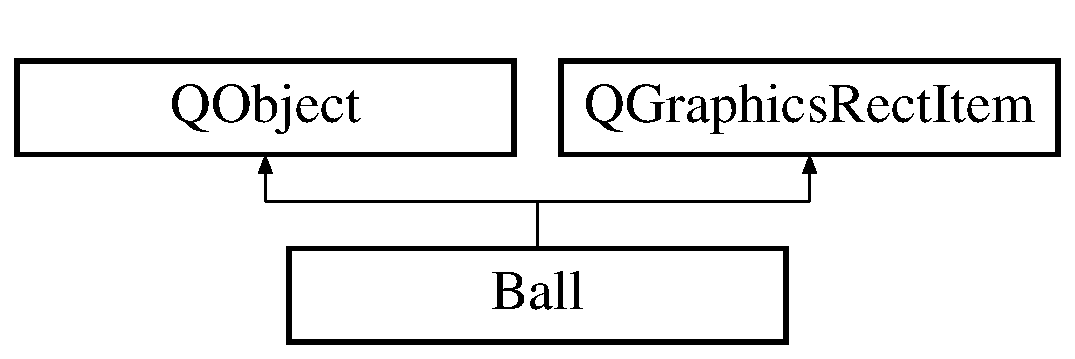
\includegraphics[height=2.000000cm]{class_ball}
\end{center}
\end{figure}
\subsection*{Public Slots}
\begin{DoxyCompactItemize}
\item 
\mbox{\Hypertarget{class_ball_a05228e822d67b25baf715cf09c325494}\label{class_ball_a05228e822d67b25baf715cf09c325494}} 
void {\bfseries move} ()
\end{DoxyCompactItemize}
\subsection*{Public Member Functions}
\begin{DoxyCompactItemize}
\item 
\hyperlink{class_ball_a773ee84b48270ddae97d29ed218f5d89}{Ball} (Q\+Graphics\+Item $\ast$parent=0)
\begin{DoxyCompactList}\small\item\em Constructor. \end{DoxyCompactList}\item 
\mbox{\Hypertarget{class_ball_ae4cbca5159194fd4f91036c34d217868}\label{class_ball_ae4cbca5159194fd4f91036c34d217868}} 
double {\bfseries get\+CenterX} ()
\end{DoxyCompactItemize}


\subsection{Detailed Description}
Die \hyperlink{class_ball}{Ball} class. 

Die \hyperlink{class_ball}{Ball} class ist für \hyperlink{class_ball}{Ball} ,zu erstellen \begin{DoxyAuthor}{Author}
Lhabib Lachil 
\end{DoxyAuthor}
\begin{DoxyVersion}{Version}
1.\+0 
\end{DoxyVersion}
\begin{DoxyDate}{Date}
26.\+01.\+2019 
\end{DoxyDate}


\subsection{Constructor \& Destructor Documentation}
\mbox{\Hypertarget{class_ball_a773ee84b48270ddae97d29ed218f5d89}\label{class_ball_a773ee84b48270ddae97d29ed218f5d89}} 
\index{Ball@{Ball}!Ball@{Ball}}
\index{Ball@{Ball}!Ball@{Ball}}
\subsubsection{\texorpdfstring{Ball()}{Ball()}}
{\footnotesize\ttfamily Ball\+::\+Ball (\begin{DoxyParamCaption}\item[{Q\+Graphics\+Item $\ast$}]{parent = {\ttfamily 0} }\end{DoxyParamCaption})}



Constructor. 


\begin{DoxyParams}{Parameters}
{\em parent} & -\/ null für standardmäßig \\
\hline
\end{DoxyParams}


The documentation for this class was generated from the following files\+:\begin{DoxyCompactItemize}
\item 
C\+:/\+Users/habib/\+Documents/sans\+\_\+titre2/ball.\+h\item 
C\+:/\+Users/habib/\+Documents/sans\+\_\+titre2/ball.\+cpp\end{DoxyCompactItemize}

\hypertarget{class_block}{}\section{Block Class Reference}
\label{class_block}\index{Block@{Block}}


Die \hyperlink{class_block}{Block} class.  




{\ttfamily \#include $<$block.\+h$>$}

Inheritance diagram for Block\+:\begin{figure}[H]
\begin{center}
\leavevmode
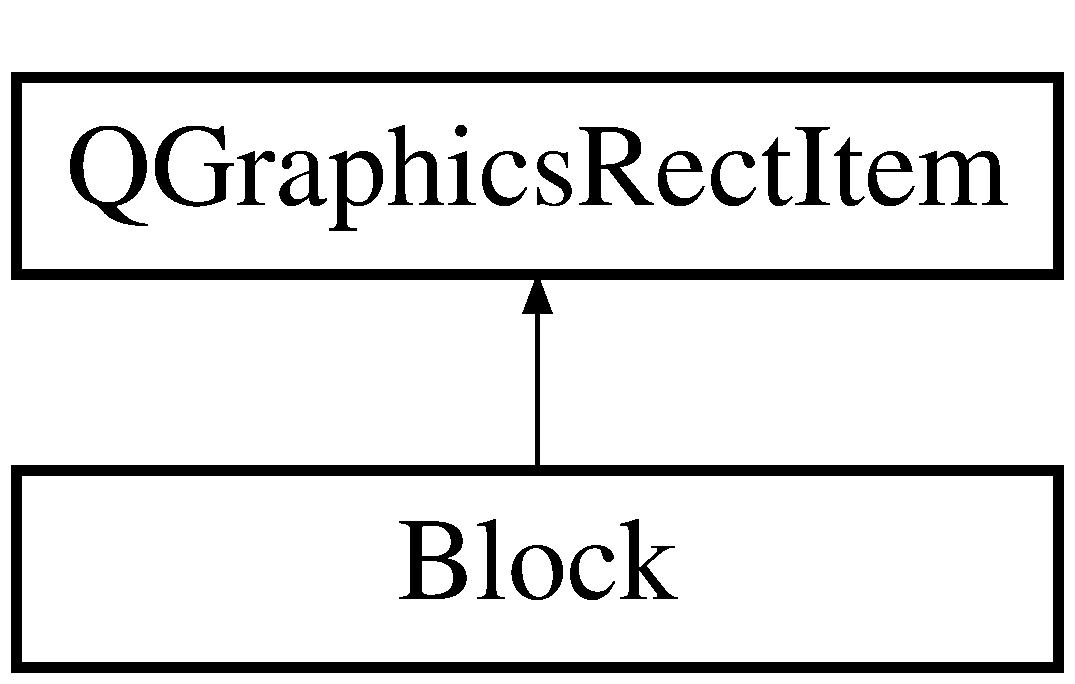
\includegraphics[height=2.000000cm]{class_block}
\end{center}
\end{figure}
\subsection*{Public Member Functions}
\begin{DoxyCompactItemize}
\item 
\hyperlink{class_block_a2577ea15ea83c909f9519842fa160fd0}{Block} (Q\+Graphics\+Item $\ast$parent=0)
\begin{DoxyCompactList}\small\item\em Constructor. \end{DoxyCompactList}\end{DoxyCompactItemize}


\subsection{Detailed Description}
Die \hyperlink{class_block}{Block} class. 

Die \hyperlink{class_ball}{Ball} class ist für \hyperlink{class_block}{Block} ,zu erstellen \begin{DoxyAuthor}{Author}
Lhabib Lachil 
\end{DoxyAuthor}
\begin{DoxyVersion}{Version}
1.\+0 
\end{DoxyVersion}
\begin{DoxyDate}{Date}
26.\+01.\+2019 
\end{DoxyDate}


\subsection{Constructor \& Destructor Documentation}
\mbox{\Hypertarget{class_block_a2577ea15ea83c909f9519842fa160fd0}\label{class_block_a2577ea15ea83c909f9519842fa160fd0}} 
\index{Block@{Block}!Block@{Block}}
\index{Block@{Block}!Block@{Block}}
\subsubsection{\texorpdfstring{Block()}{Block()}}
{\footnotesize\ttfamily Block\+::\+Block (\begin{DoxyParamCaption}\item[{Q\+Graphics\+Item $\ast$}]{parent = {\ttfamily 0} }\end{DoxyParamCaption})}



Constructor. 


\begin{DoxyParams}{Parameters}
{\em parent} & -\/ null für standardmäßig\\
\hline
\end{DoxyParams}
Diese methode ist für \hyperlink{class_block}{Block} \char`\"{}\+Circle oder  Triangle oder Circle zu erstellen\char`\"{} 

The documentation for this class was generated from the following files\+:\begin{DoxyCompactItemize}
\item 
C\+:/\+Users/habib/\+Documents/sans\+\_\+titre2/block.\+h\item 
C\+:/\+Users/habib/\+Documents/sans\+\_\+titre2/block.\+cpp\end{DoxyCompactItemize}

\hypertarget{class_game}{}\section{Game Class Reference}
\label{class_game}\index{Game@{Game}}


Die \hyperlink{class_game}{Game} class.  




{\ttfamily \#include $<$game.\+h$>$}

Inheritance diagram for Game\+:\begin{figure}[H]
\begin{center}
\leavevmode
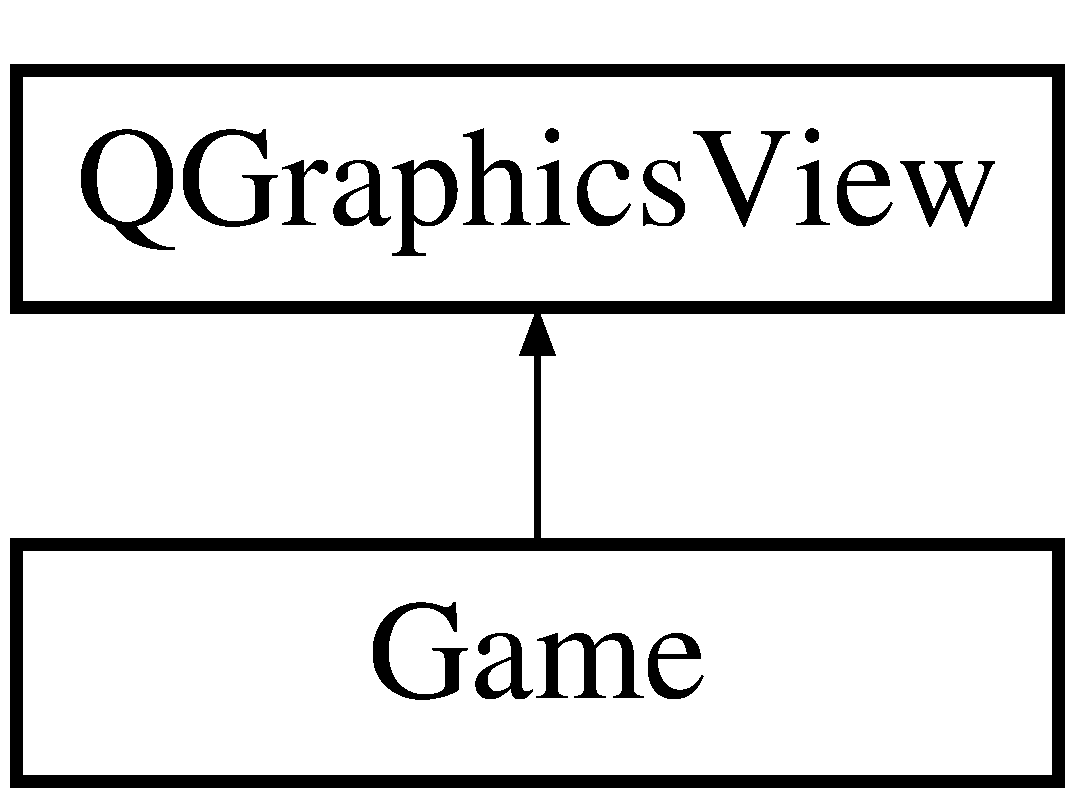
\includegraphics[height=2.000000cm]{class_game}
\end{center}
\end{figure}
\subsection*{Public Member Functions}
\begin{DoxyCompactItemize}
\item 
\hyperlink{class_game_a32d7e09112c37ff84736ea797c1eb7f0}{Game} (Q\+Widget $\ast$parent=N\+U\+LL)
\begin{DoxyCompactList}\small\item\em Constructor. \end{DoxyCompactList}\item 
\mbox{\Hypertarget{class_game_a3d9b98f7c4a96ecf578f75b96c9f0e90}\label{class_game_a3d9b98f7c4a96ecf578f75b96c9f0e90}} 
void \hyperlink{class_game_a3d9b98f7c4a96ecf578f75b96c9f0e90}{start} ()
\begin{DoxyCompactList}\small\item\em Diese methode ist für " ball und paddle und blocks zu erstellen. \end{DoxyCompactList}\item 
\mbox{\Hypertarget{class_game_ae4d31cfbf571bb1239f9614099614f2f}\label{class_game_ae4d31cfbf571bb1239f9614099614f2f}} 
void {\bfseries create\+Block\+Col} (double x)
\item 
\mbox{\Hypertarget{class_game_a029fabc7b925001939b1b956ba30df14}\label{class_game_a029fabc7b925001939b1b956ba30df14}} 
void {\bfseries creat\+Block\+Grid} ()
\end{DoxyCompactItemize}
\subsection*{Public Attributes}
\begin{DoxyCompactItemize}
\item 
\mbox{\Hypertarget{class_game_a8119e3b9a632906c6808fa294b46a92a}\label{class_game_a8119e3b9a632906c6808fa294b46a92a}} 
Q\+Graphics\+Scene $\ast$ {\bfseries scene}
\end{DoxyCompactItemize}


\subsection{Detailed Description}
Die \hyperlink{class_game}{Game} class. 

Die \hyperlink{class_game}{Game} class ist für \hyperlink{class_game}{Game}\char`\"{}\+Block und Ball Paddle im Scene zu leigen \char`\"{},zu erstellen \begin{DoxyAuthor}{Author}
Lhabib Lachil 
\end{DoxyAuthor}
\begin{DoxyVersion}{Version}
1.\+0 
\end{DoxyVersion}
\begin{DoxyDate}{Date}
26.\+01.\+2019 
\end{DoxyDate}


\subsection{Constructor \& Destructor Documentation}
\mbox{\Hypertarget{class_game_a32d7e09112c37ff84736ea797c1eb7f0}\label{class_game_a32d7e09112c37ff84736ea797c1eb7f0}} 
\index{Game@{Game}!Game@{Game}}
\index{Game@{Game}!Game@{Game}}
\subsubsection{\texorpdfstring{Game()}{Game()}}
{\footnotesize\ttfamily Game\+::\+Game (\begin{DoxyParamCaption}\item[{Q\+Widget $\ast$}]{parent = {\ttfamily NULL} }\end{DoxyParamCaption})\hspace{0.3cm}{\ttfamily [inline]}}



Constructor. 


\begin{DoxyParams}{Parameters}
{\em parent} & -\/ null für standardmäßig\\
\hline
\end{DoxyParams}
Diese methode ist für \hyperlink{class_game}{Game} zu erstellen 

The documentation for this class was generated from the following file\+:\begin{DoxyCompactItemize}
\item 
C\+:/\+Users/habib/\+Documents/sans\+\_\+titre2/game.\+h\end{DoxyCompactItemize}

\hypertarget{class_main_window}{}\section{Main\+Window Class Reference}
\label{class_main_window}\index{Main\+Window@{Main\+Window}}
Inheritance diagram for Main\+Window\+:\begin{figure}[H]
\begin{center}
\leavevmode
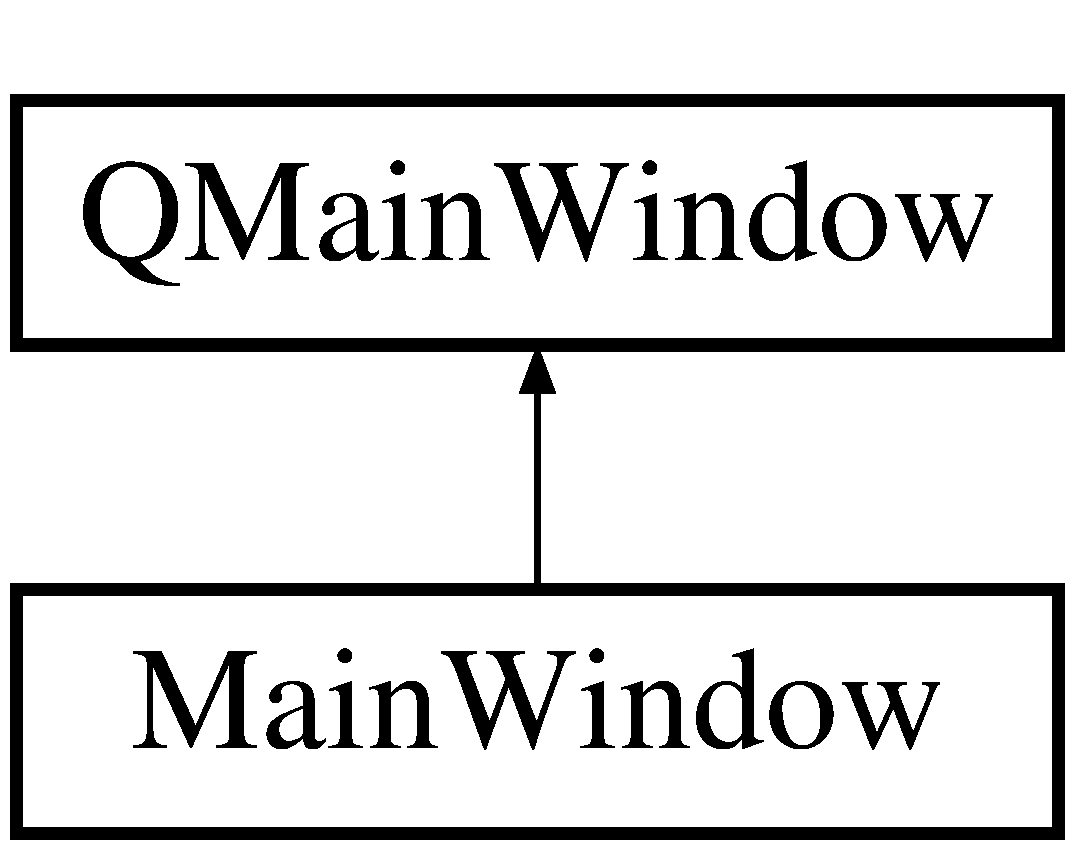
\includegraphics[height=2.000000cm]{class_main_window}
\end{center}
\end{figure}
\subsection*{Public Member Functions}
\begin{DoxyCompactItemize}
\item 
\mbox{\Hypertarget{class_main_window_a996c5a2b6f77944776856f08ec30858d}\label{class_main_window_a996c5a2b6f77944776856f08ec30858d}} 
{\bfseries Main\+Window} (Q\+Widget $\ast$parent=nullptr)
\end{DoxyCompactItemize}


The documentation for this class was generated from the following files\+:\begin{DoxyCompactItemize}
\item 
C\+:/\+Users/habib/\+Documents/sans\+\_\+titre2/mainwindow.\+h\item 
C\+:/\+Users/habib/\+Documents/sans\+\_\+titre2/mainwindow.\+cpp\end{DoxyCompactItemize}

\hypertarget{class_paddle}{}\section{Paddle Class Reference}
\label{class_paddle}\index{Paddle@{Paddle}}


Die \hyperlink{class_ball}{Ball} class.  




{\ttfamily \#include $<$paddle.\+h$>$}

Inheritance diagram for Paddle\+:\begin{figure}[H]
\begin{center}
\leavevmode
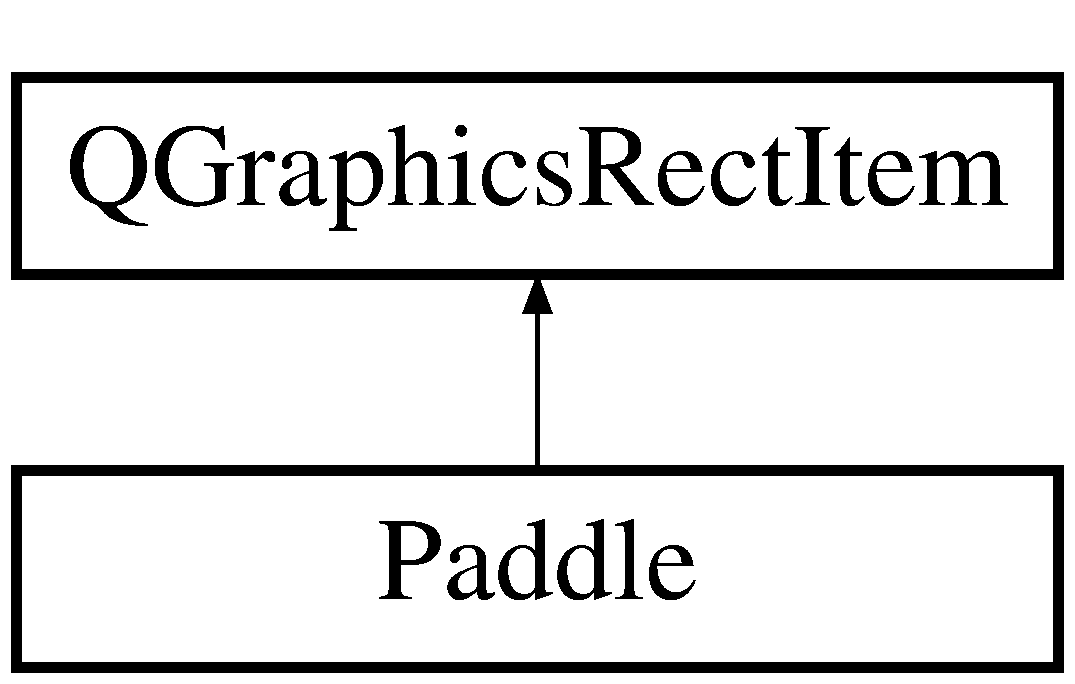
\includegraphics[height=2.000000cm]{class_paddle}
\end{center}
\end{figure}
\subsection*{Public Member Functions}
\begin{DoxyCompactItemize}
\item 
\hyperlink{class_paddle_ab8dfa8e73e79ae577fcd90bc7016aef0}{Paddle} (Q\+Graphics\+Item $\ast$parent=0)
\begin{DoxyCompactList}\small\item\em Constructor. \end{DoxyCompactList}\item 
\mbox{\Hypertarget{class_paddle_ad6f95463e709f2d915403813071a3a17}\label{class_paddle_ad6f95463e709f2d915403813071a3a17}} 
double \hyperlink{class_paddle_ad6f95463e709f2d915403813071a3a17}{get\+CenterX} ()
\begin{DoxyCompactList}\small\item\em public methods für get\+CenterX \end{DoxyCompactList}\item 
\mbox{\Hypertarget{class_paddle_aa66dccdb50eef525d75e2f9ddae4f449}\label{class_paddle_aa66dccdb50eef525d75e2f9ddae4f449}} 
void \hyperlink{class_paddle_aa66dccdb50eef525d75e2f9ddae4f449}{mouse\+Move\+Event} (Q\+Graphics\+Scene\+Mouse\+Event $\ast$event)
\begin{DoxyCompactList}\small\item\em public methods für events von mouse \end{DoxyCompactList}\end{DoxyCompactItemize}


\subsection{Detailed Description}
Die \hyperlink{class_ball}{Ball} class. 

Die \hyperlink{class_ball}{Ball} class ist für \hyperlink{class_paddle}{Paddle} ,zu erstellen \begin{DoxyAuthor}{Author}
Lhabib Lachil 
\end{DoxyAuthor}
\begin{DoxyVersion}{Version}
1.\+0 
\end{DoxyVersion}
\begin{DoxyDate}{Date}
26.\+01.\+2019 
\end{DoxyDate}


\subsection{Constructor \& Destructor Documentation}
\mbox{\Hypertarget{class_paddle_ab8dfa8e73e79ae577fcd90bc7016aef0}\label{class_paddle_ab8dfa8e73e79ae577fcd90bc7016aef0}} 
\index{Paddle@{Paddle}!Paddle@{Paddle}}
\index{Paddle@{Paddle}!Paddle@{Paddle}}
\subsubsection{\texorpdfstring{Paddle()}{Paddle()}}
{\footnotesize\ttfamily Paddle\+::\+Paddle (\begin{DoxyParamCaption}\item[{Q\+Graphics\+Item $\ast$}]{parent = {\ttfamily 0} }\end{DoxyParamCaption})}



Constructor. 


\begin{DoxyParams}{Parameters}
{\em parent} & -\/ null für standardmäßig\\
\hline
\end{DoxyParams}
Diese methode ist für \hyperlink{class_paddle}{Paddle} zu erstellen 

The documentation for this class was generated from the following files\+:\begin{DoxyCompactItemize}
\item 
C\+:/\+Users/habib/\+Documents/sans\+\_\+titre2/paddle.\+h\item 
C\+:/\+Users/habib/\+Documents/sans\+\_\+titre2/paddle.\+cpp\end{DoxyCompactItemize}

%--- End generated contents ---

% Index
\backmatter
\newpage
\phantomsection
\clearemptydoublepage
\addcontentsline{toc}{chapter}{Index}
\printindex

\end{document}
